%--------------------------------------------------------------------
%\chapter{Topic Models}
%--------------------------------------------------------------------

The BuitenBeter dataset consists of 13,811 geo-tagged issues reported to the
office of public order in the Netherlands between July and September 2012.  Each
issue is assigned to one of 16 categories such as "poor road conditions", "Dirt
on the street" or "Graffiti".

Geographical co-occurrences of arbitrary categorical observations - such as
public order issues of the BuitenBeter dataset - can be used to discover latent
underlying factors that explain observations which co-occur more frequently than
expected by chance.  One method for detecting these latent factors is
probabilistic topic modelling, where grouped observations are modelled as being
sampled from mixtures of latent topics, which are probability distributions over
the set of distinct observations.

For the BuitenBeter dataset, we e.g. might expect that areas where graffities
are reported will see many reports of the category "Dirt on the street" since
both categories are related to urban environments. We model those environments
as hidden "topics".
  
Existing approaches for geographical topic modelling adopt topic models such as
latent Dirichlet allocation \cite{Blei:2003:LDA:944919.944937} and extend the
models by assigning distributions over locations to topics, or by introducing
latent geographical regions. In models which extend topics for spatial
distributions (such as two-dimensional normal distributions)
\cite{conf/wsdm/Sizov10}, topics with a complex (i.e. non-Gaussian) spatial
distribution cannot be detected. In models with latent, Gaussian distributed
regions \cite{conf/www/YinCHZH11}, documents within a complex shaped topic area
do not influence the topic distribution of distant documents within the same
area. Therefore, topics with a complex spatial distribution such as topics
distributed along coastlines, rivers or country borders are harder to detect by
such methods.  More elaborate models introduce artificial assumptions about the
structure of geographical distributions, e.g. by introducing hierarchical
structures \cite{ahmed13} in advance.
%Additionally, some approaches \cite{conf/www/MeiLSZ06,conf/www/YinCHZH11} do not model document-specific
%topic distributions. 

We introduce a novel geographical topic model which captures dependencies
between geographical regions to support the detection of topics with complex,
e.g. non-Gaus\-sian distributed spatial structures \cite{CCK1}.
%The model is based on a hierarchical Dirichlet process
%extended to support multiple base distributions, which we name MDP. 
%Our method thus is called the MDP-based geographical topic model (MGTM). 
%We use the MDP to dynamically smooth topic distributions between groups of spatially
%adjacent documents.

Our model differs from existing approaches in several aspects:

We model locations and words separately, as the separation of spatial clusters
and document semantics allows us to define meaningful neighbour relations
between spatially adjacent clusters. Our topic model takes a set of geographical
clusters as input.

We also expect that geographical clusters adjacent in space exhibit similar
topic distributions: Most geographical topics cannot be approximated by a simple
spatial probability distribution such as a Gaussian distribution and for these
complex topic areas, coherent sets of multiple spatial distributions are a
reasonable approximation.  Therefore we detect and smooth the topic distribution
of these adjacent regions to increase the probability of detecting coherent
topic areas.

The detection of geographical clusters is straight-forward: We use a mixture of
a fixed number of Fisher distributions -- distributions on a three dimensional
unit sphere similar to isotropic Gaussian distributions on a plane. The
parameters are fit using the approximation given by Banerjee et
al.~\cite{DBLP:journals/jmlr/BanerjeeDGS05} in an expectation-maximisation
algorithm.  In our model, each cluster is associated with a distribution over
the set of topics, sampled from a Dirichlet process (DP) with a common base
measure which is itself drawn from a DP with Dirichlet distributed multinomial
distributions over the set of categories as base measure.  For the smoothing of
topic distributions of adjacent clusters, we first define the adjacency relation
using the Delaunay triangulation \cite{journals/csur/Aurenhammer91} of the
cluster centroids.  Each public order issue report draws an own topic
distribution from a DP with a weighted mixture of the topic distribution of its
own geographical cluster and its neighbour clusters as base measure.  Finally,
each observed report category is drawn from its document-specific topic
distribution.  For a detailed description of the model and its parameters, we
refer to our paper \cite{CCK1}.

To train our model on the BuitenBeter dataset, we use 300 clusters and the
initial settings for the parameters $\beta = 0.5$, $\gamma = 1.0$, $\alpha_0 =
1.0$, $A = 99999$, $\delta = 1.0$. By setting $A$ to such a high value, we give
up document-specific topic distributions and sample the categories directly from
a mixture of region-specific topic distributions. All other parameters are set
to the values used in the paper \cite{CCK1}, except for the hyperparameters for
$A$, which is fixed.

For creating a comprehensible report, the detected topics can be characterised
by their most-likely categories:

Topic 1: \textit{Dirt on the street}, \ \textit{Other}, \ \textit{Graffities\\}
Topic 2: \textit{Damaged street light}, \ \textit{Bad road}\\
Topic 3: \textit{Obstacle by trees}, \ \textit{Weed}, \ \textit{Loose paving stones}, \ \textit{Bad road}, \ \textit{Idea/wish}\\
Topic 4: \textit{Other}, \ \textit{Weed}, \ \textit{Loose paving stones}, \ \textit{Bad road}, \ \textit{Damaged street light}, \ \textit{Idea/wish}


%for reduzing the size, set the width to 0.22\textwid
\begin{figure}[]
\centering
\subfigure[Topic 1]{
  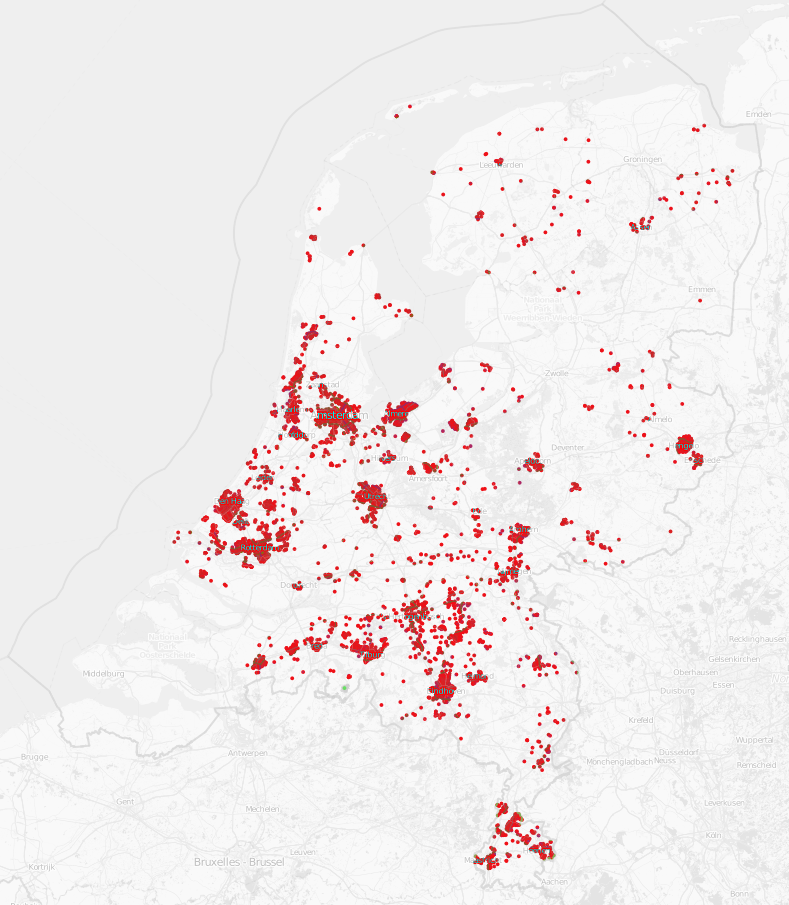
\includegraphics[width=0.3\textwidth,natwidth=556.19,natheight=432]{img/map/1.png}
  \label{plot:act20}
  \setcounter{subfigure}{1}
} 
\subfigure[Topic 2]{
  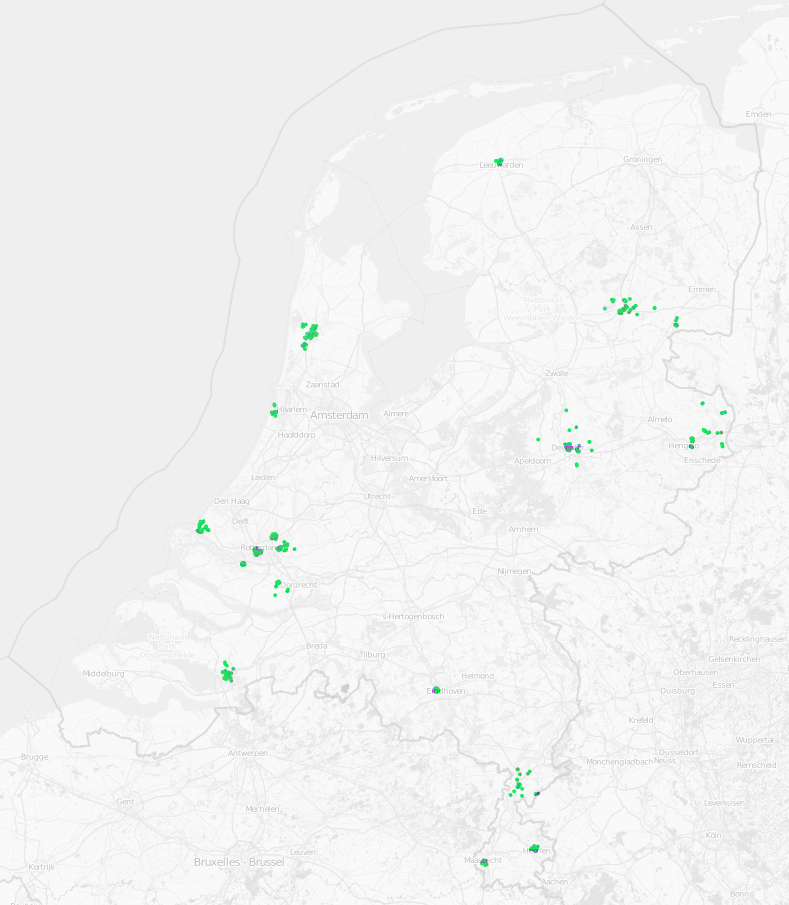
\includegraphics[width=0.3\textwidth,natwidth=556.19,natheight=432]{img/map/2.png}
  \label{plot:act20}
  \setcounter{subfigure}{2}
}

\subfigure[Topic 3]{
  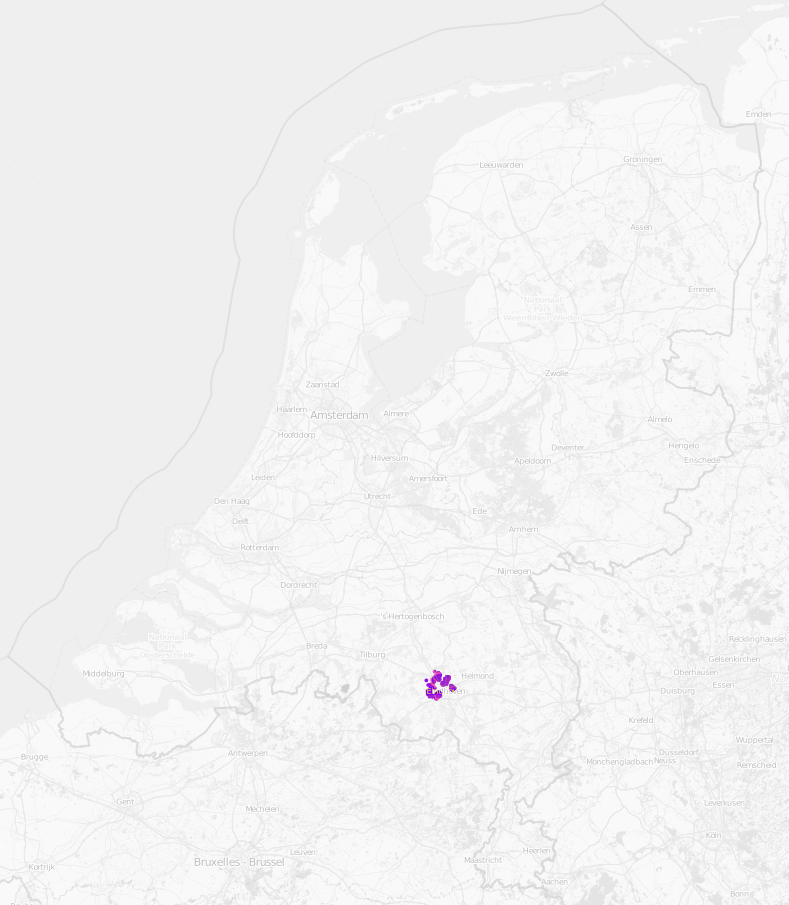
\includegraphics[width=0.3\textwidth,natwidth=556.19,natheight=432]{img/map/3.png}
  \label{plot:act20}
  \setcounter{subfigure}{3}
}
\subfigure[Topic 4]{
  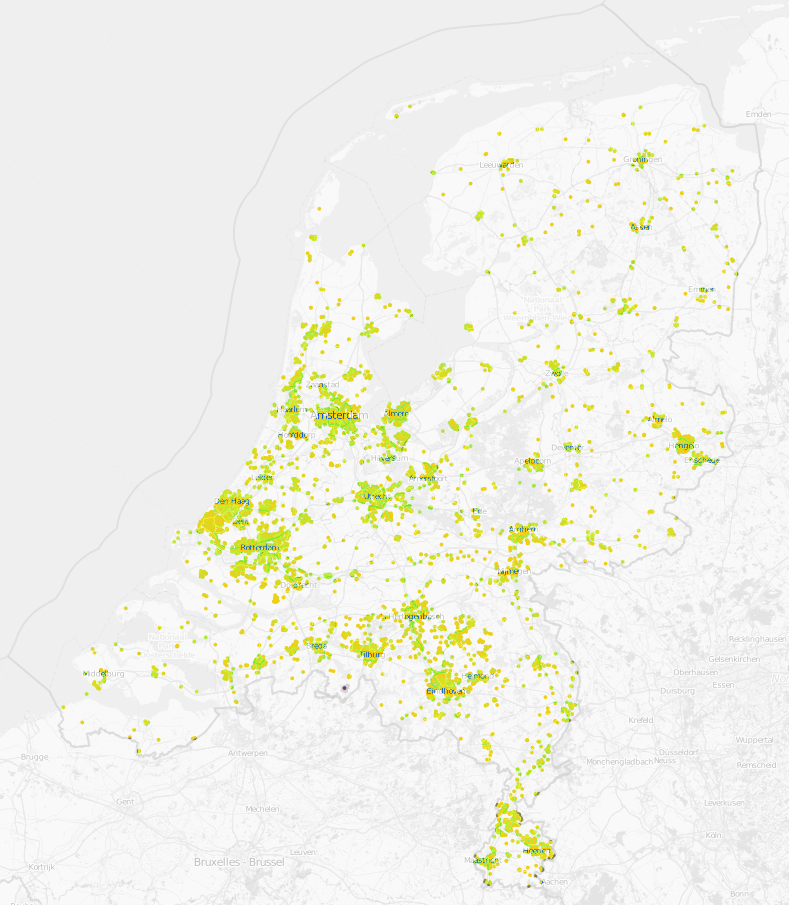
\includegraphics[width=0.3\textwidth,natwidth=556.19,natheight=432]{img/map/4.png}
  \label{plot:act20}
  \setcounter{subfigure}{4}
} 

\caption{
  Document positions of reports with above-average probabilities for Topic 1-4 on the map of the Netherlands.
}
\label{fig:netmaps}
\end{figure}

The position of documents with an above-average probability for each topic are
shown in \vbox{Figure \ref{fig:netmaps}}.  We see that, as expected, Topic 1 is
only observed in the area of larger cities, whilst Topic 4 is present across the
whole country.  Topic 2 occurs mostly within city centres.  Topic 3 is observed
in the area of Eindhoven for which different categories were available in the
BuitenBeter application.

%%% Local Variables: 
%%% mode: latex
%%% TeX-master: "../D1-2"
%%% End: 
